\section{Additional Visual Evidence}\label{sec:visual_appendix}
Figures in this section retain the historical January PM2.5 pilot (30 fields, seven clear events). They are exploratory controls; current annual PM2.5 metrics and complete maps appear in the numeric tables and Supplement S10. No pilot rate is used as an annual result. The following figures complement the main tables with the retained primary anchor-based motion and extremum-based geometry diagnostics. Their displayed ME percentages are 100 times the decimal rates used in the main table. Standard centroid-based SNS, TW, and canvas-normalized TD remain in Supplement S3.

\subsection{Local Witnesses and the Absolute-Reference Control}
\begin{figure}[H]\centering
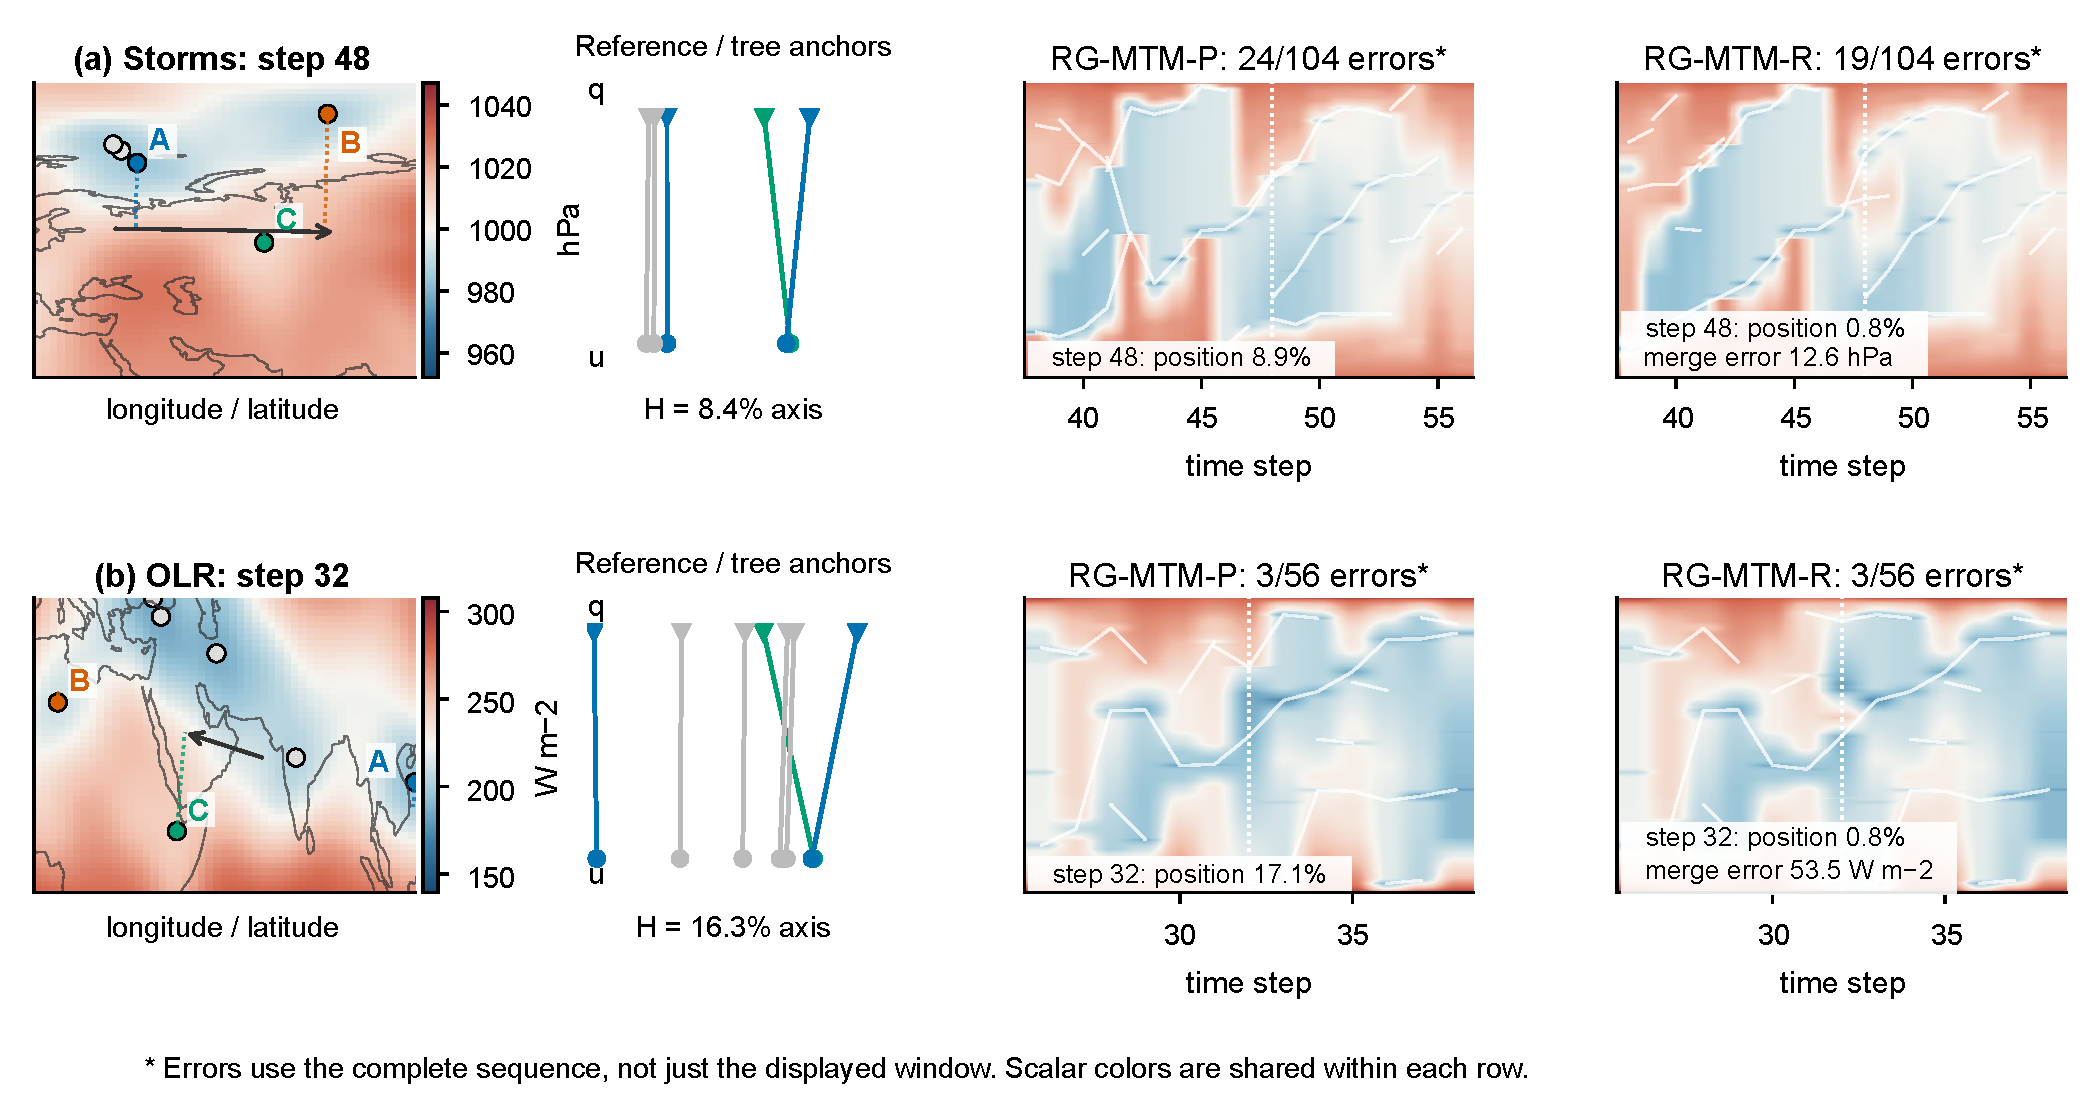
\includegraphics[width=\linewidth]{figures/rgmtm_linked_cases.pdf}
\caption{Local Storms and OLR witnesses retained from the previous integrated revision. Source fields, reference-to-anchor links, and P/R windows explain the individual hierarchy conflicts. Local labels report maximum anchor error and scalar cost; map titles give complete-sequence motion-proxy counts. Storms is the frame-48 example in the main introduction; OLR is the retained frame-32 example.}
\label{fig:s_local_witnesses}\end{figure}
The independent absolute-reference control is shown in main-paper Fig.~6. Section~\ref{sec:bisector_protocol} gives its protocol, calibration, and measurements; Fig.~\ref{fig:s_full_bisector_three_methods} retains the full visual comparison.
\clearpage
\subsection{Motion Errors and Scalar Costs}
\begin{figure}[H]\centering
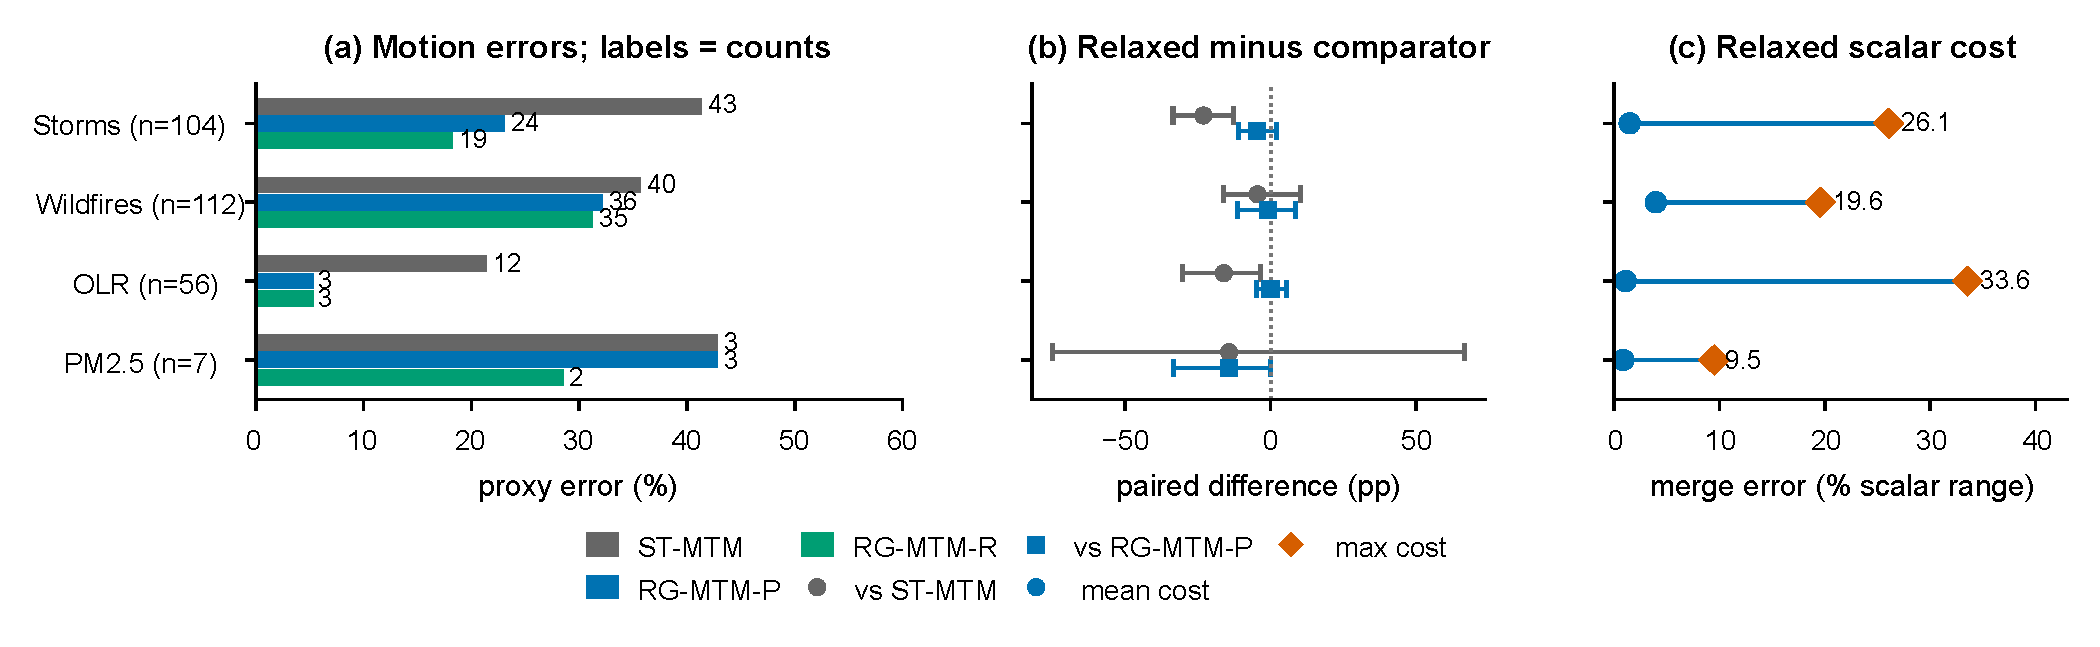
\includegraphics[width=\linewidth]{figures/rgmtm_motion_scalar_cost.pdf}
\caption{Four real sequences: primary motion-error counts and rates, paired relaxed-minus-comparator differences with retained temporal-block 95\% intervals, and relaxed mean/maximum scalar costs. The reference protocol fixes a two-step window and 2\% thresholds; PM2.5 has seven clear events. Scalar costs in this drawing use the saved fixed-order optimum; measured raster values agree to the numerical tolerance reported in the main text.}
\label{fig:s_motion_cost}\end{figure}
\begin{figure}[H]\centering
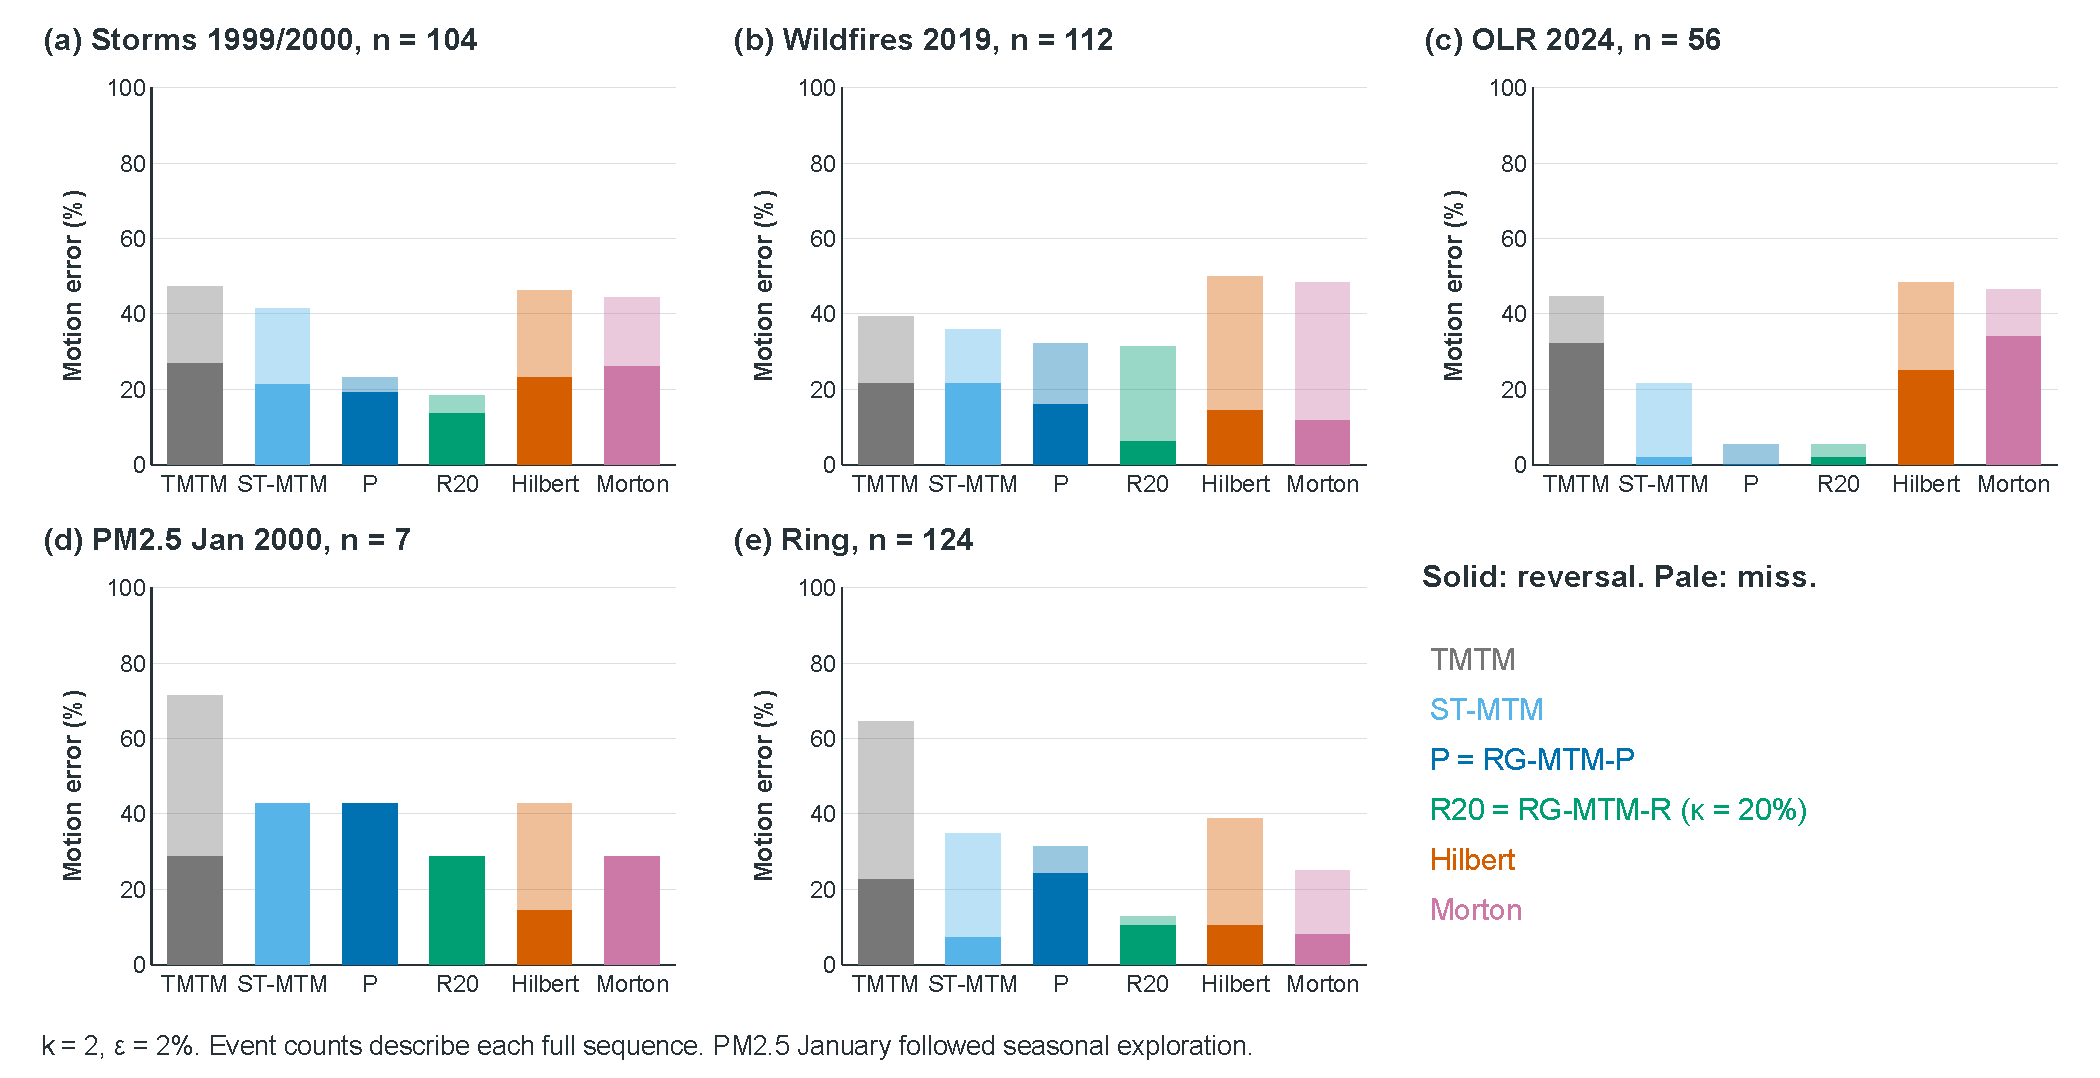
\includegraphics[width=\linewidth]{figures/rgmtm_motion_error_comparison.pdf}
\caption{Primary motion errors decomposed into reversals and misses across five sequences and the native curve controls. Solid portions show reversals and hatched portions show misses. Denominators are the shared clear two-dimensional events.}
\label{fig:s_motion_errors}\end{figure}

\subsection{Geometric Neighbourhoods}
\begin{figure}[H]\centering
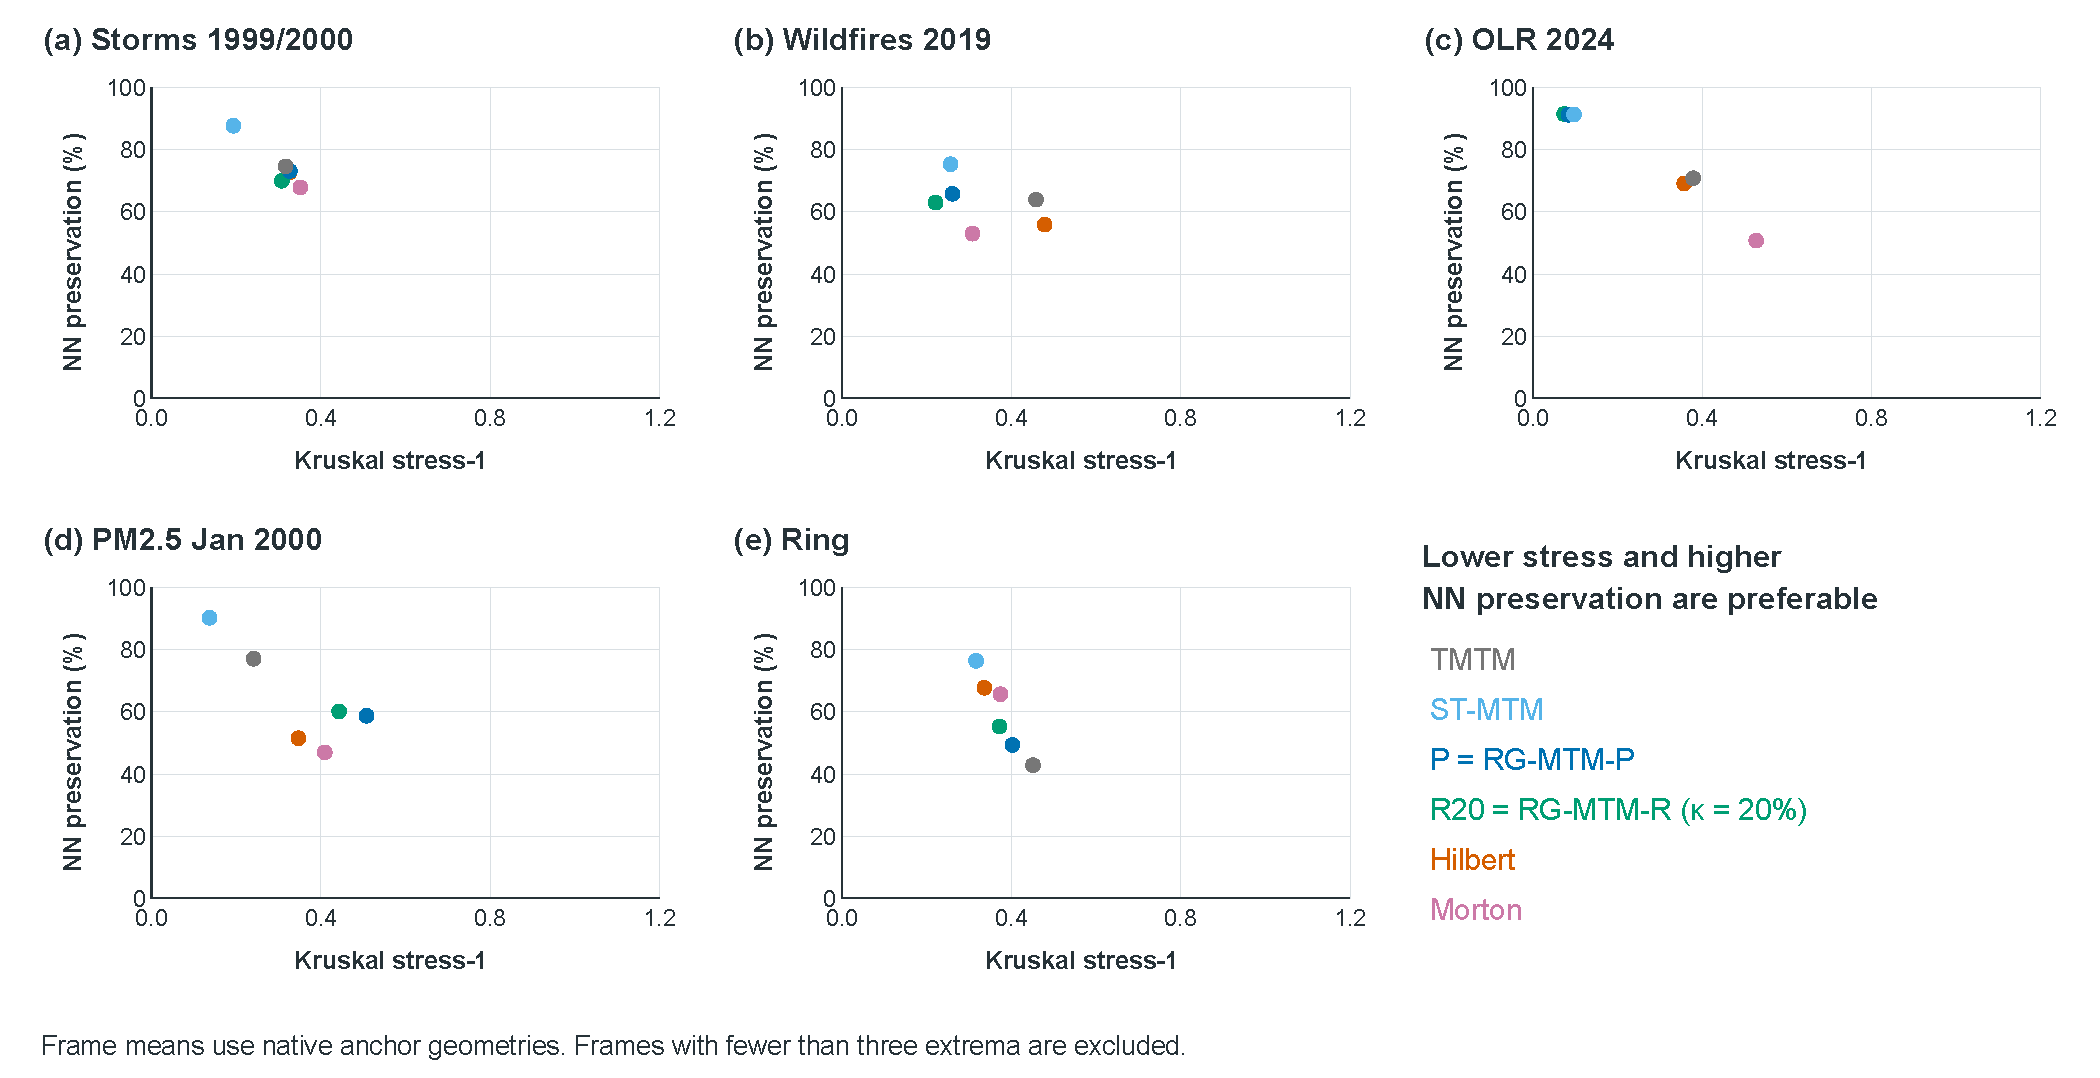
\includegraphics[width=\linewidth]{figures/rgmtm_neighbourhood_preservation.pdf}
\caption{Retained extremum-based stress-1 and nearest-neighbour identity preservation on frames with at least three extrema. Each method keeps its own anchor geometry. These metrics use different definitions from SNS and TW, whose complete values and eligible-frame counts are reported in Supplement S3.}
\label{fig:s_neighbours}\end{figure}

\subsection{Window Sensitivity}
\begin{figure}[H]\centering
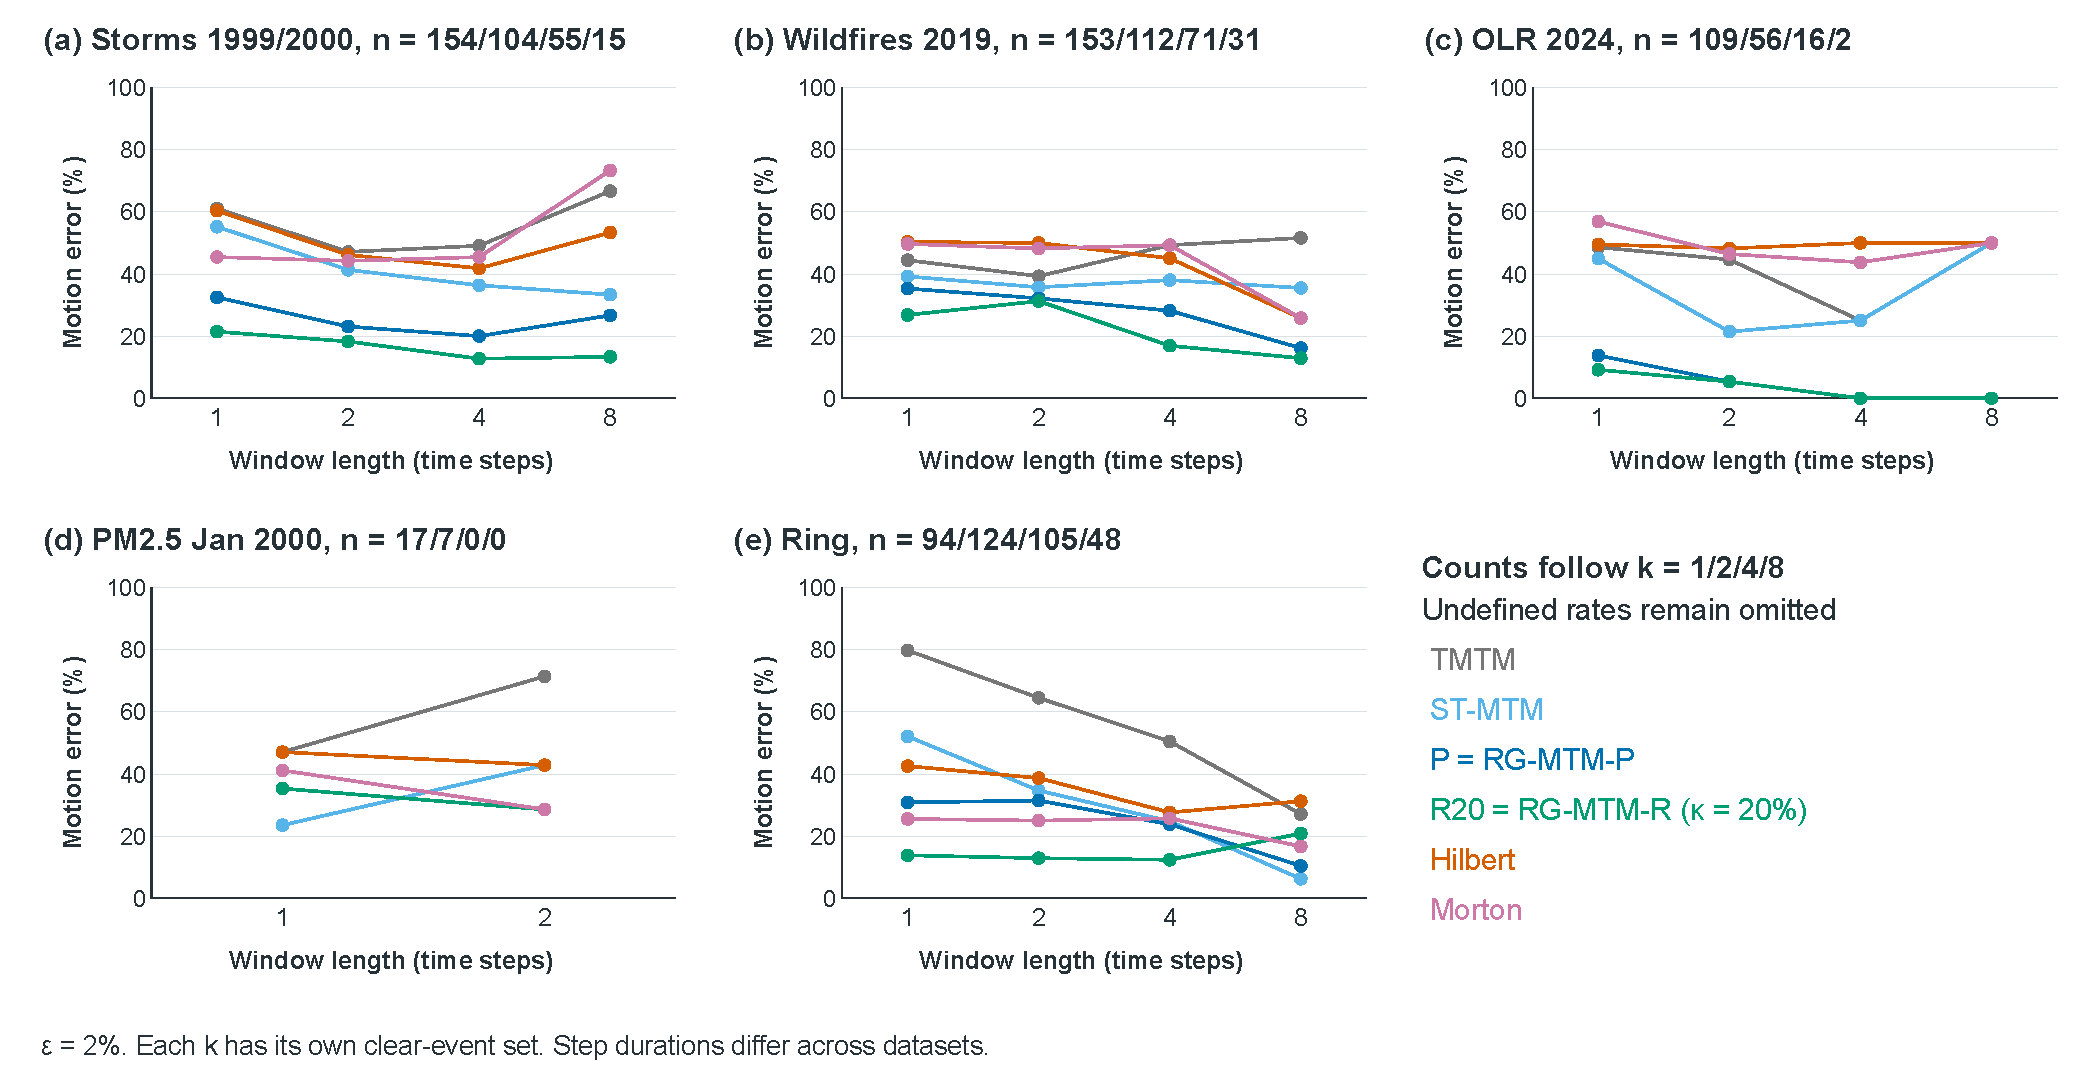
\includegraphics[width=\linewidth]{figures/rgmtm_motion_window_sensitivity.pdf}
\caption{Motion error for windows of 1, 2, 4, and 8 steps at the same 2\% thresholds. Each window has its own event set, with counts shown in that order above each panel. Sampling intervals differ by dataset. Undefined rates are omitted and their event counts remain explicit.}
\label{fig:s_windows}\end{figure}

\subsection{Native Sample Traversals and Scalar Cost}
\begin{figure}[H]\centering
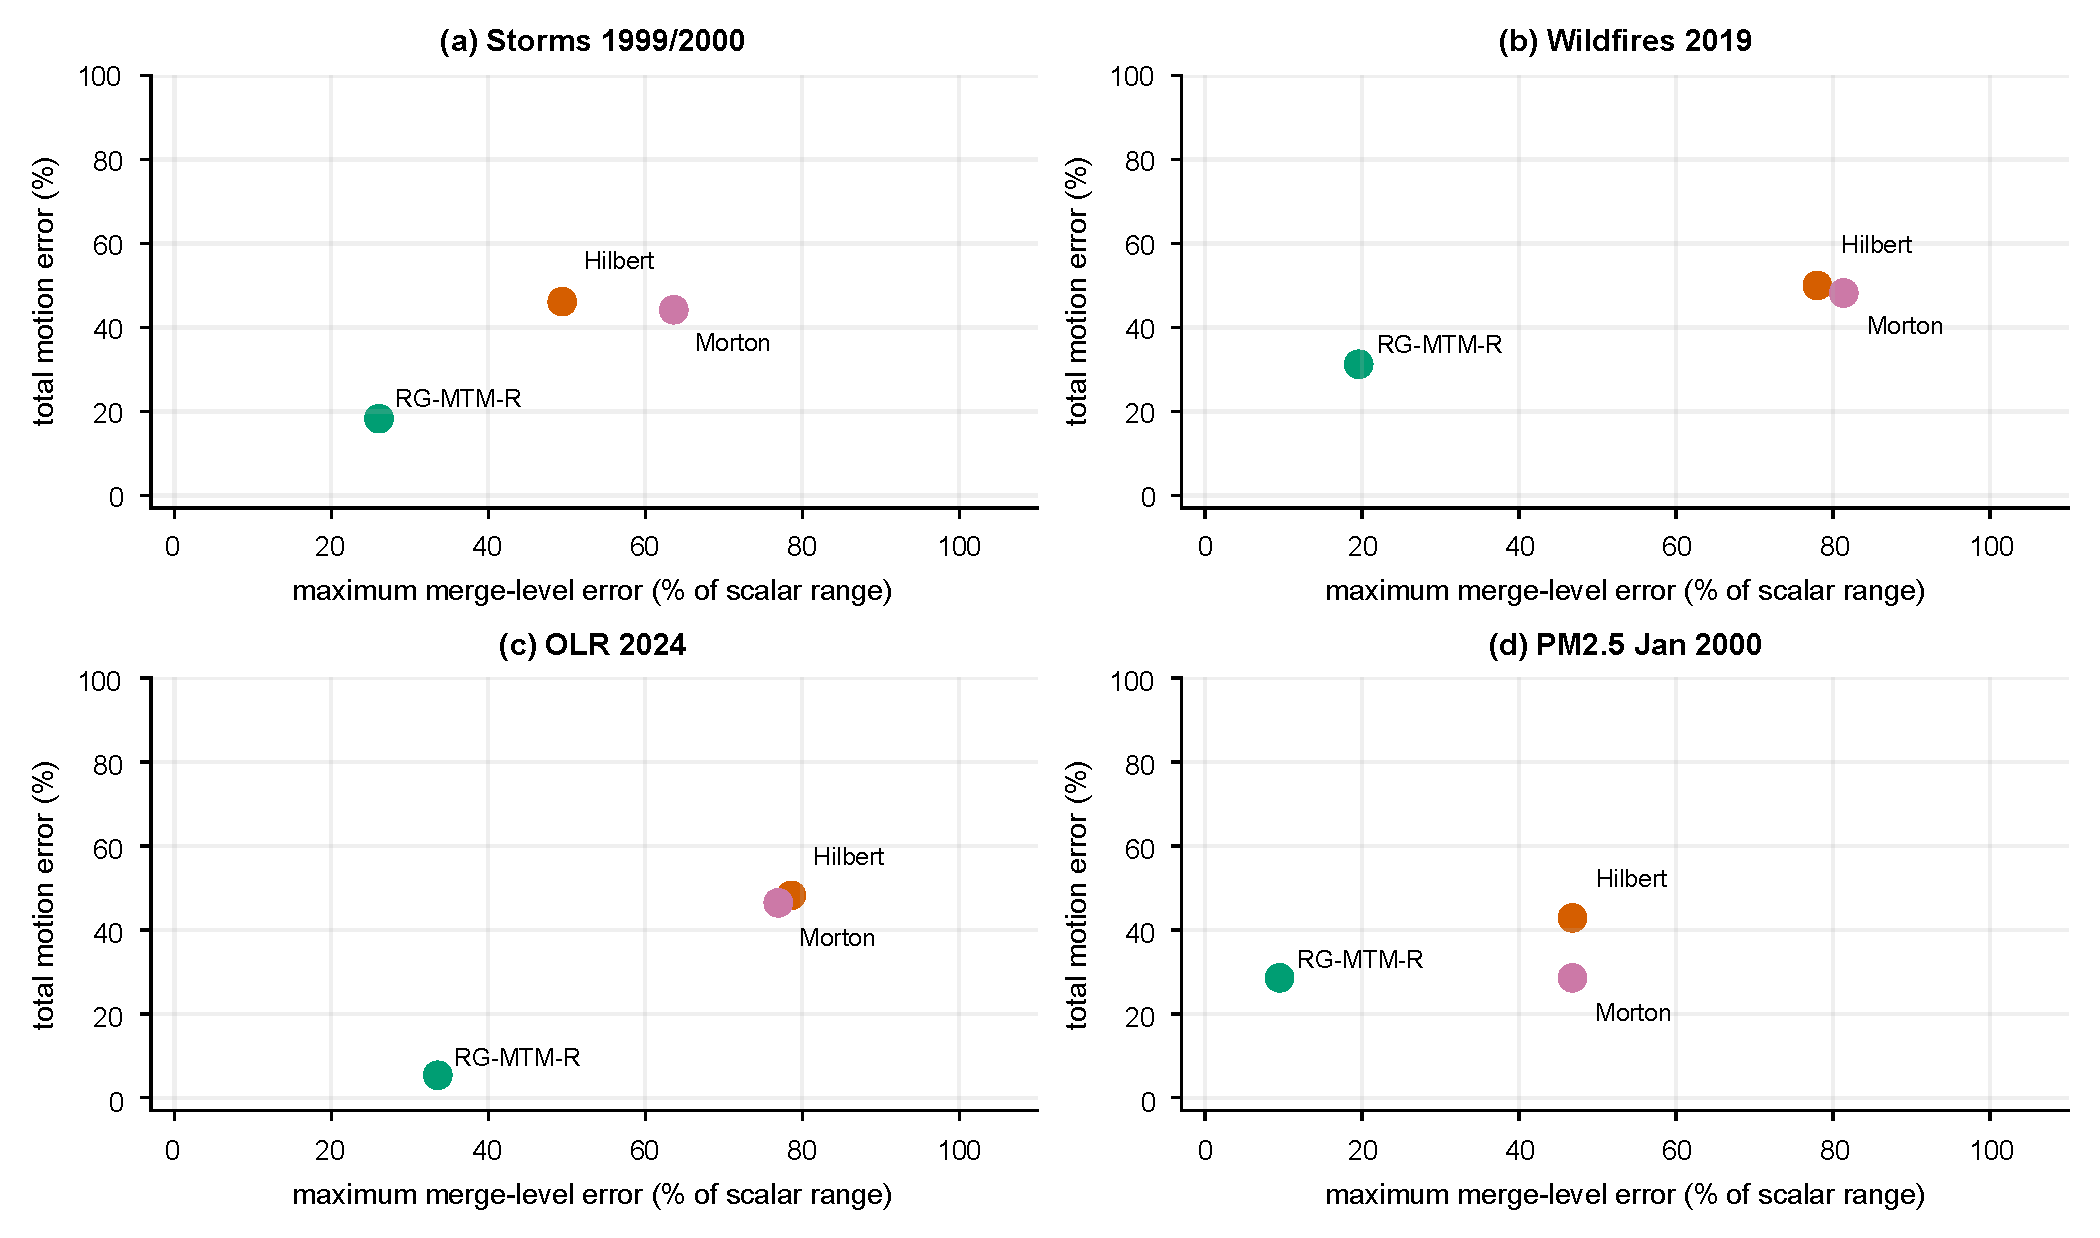
\includegraphics[width=\linewidth]{figures/rgmtm_topology_motion_tradeoff.pdf}
\caption{Motion error versus maximum merge-level distortion for RG-MTM-R and native Hilbert/Morton traversals. Each point is one fixed operating setting; native curves retain original sample values while RG-MTM-R uses optimal refilling. The comparison includes both ordering and rendering policy. Horizontal values are sequence maxima of the saved scalar-cost summaries.}
\label{fig:s_native_cost}\end{figure}
